\chapter{Collaborative filtering}

% - nel capitolo dei recommendation system parlare dei collaborative filter in modo più dettagliato e legato al progetto -








\section{Memory-based} \hfill \break
I filtri collaborativi Memory-based sono stati introdotti per via delle osservazioni che vennero fatti sugl utenti, i quali si fidano
maggiormente delle raccomandazioni di altri che la pensano allo stesso modo. Questi metodi mirano a calcolare le relazioni tra utenti
e item attraverso lo schema dei vicini che identifica sia coppie di item che tendono ad essere usati insieme o hanno un grado di 
similarità alto o utenti con uno storico di item usati simile. \cite{taxonomy-of-recommender-agents-on-the-internet}
Questi approcci divennero molto famosi grazie alla loro semplicità di implementazione, molto intuitivi, non necessitano il training e
aggiustamento di molti parametri, e l'utente può capire la ragione che sta dietro ogni raccomandazione 

Filtri collaborativi che usano metodi Memory-based (definiti anche \textit{Neighborhood-based}) possono essere classificati in altre due
categorie:


\subsection{User-based filtering} \hfill \break
Questi sistemi, definiti anche con l'acronimo UB-CF (\textit{User-based Collaborative Filter}) raccomandano una serie di item a 
un utente che utenti simili hanno usato o valutato. Questo algoritmo prima trova un valore che rappresenta la similarità tra utenti. 
E basandosi su questi valori, prende uno o più utenti tra quelli che risultano simili e raccomanda item che questi utenti simili 
hanno usato o valutato in precedenza.

Molti di questi approcci possono essere generalizzati dall'algoritmo definito dai seguenti step:
\begin{enumerate}
	\item Specificare qual'è il l'utente a cui si vuole applicare l'algoritmo di raccomandazione e recuperare quali utenti possono 
	avere dato valutazioni o usato item simili al utente target. Piuttosto che recuperare tutti gli utenti, per velocizzare l'esecuzione
	dell'algoritmo, è possibile selezionare soltanto un gruppo di utenti in modo casuale oppure associare dei valori di similarità tra 
	tutti gli utenti e confrontando questi valori con quello dell'utente target, selezionare i relativi utenti che superano una soglia
	scelta, oppure utilizzare tecniche di clustering. 
	un numero limitato per effettuare la raccomandazione, 
	\item Estrarre quegli item a cui l'utente target non ha mai interagito e per questo motivo gli possono interessare, e mostrarli 
	all'utente target.
\end{enumerate}

\begin{figure}[ht!]
	\centering
	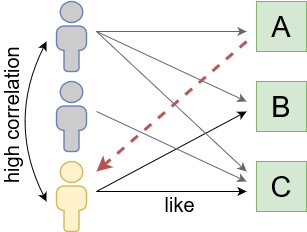
\includegraphics[scale=0.5]{images/UB_CF_ex.PNG}
	\caption{Esempio di applicazione di un sistema di raccomandazione User-based}
	\label{fig:UB_CF}
\end{figure}

Questi approcci sono facilmente implementabili, indipendenti dal contesto in cui sono applicati e possono essere più accurati rispetto
a tecniche basate sul Content-based dall'altra parte all'aumentare del numero di utenti che vado a considerare per fare le 
raccomandazioni migliore è la precisione di questo processo ma anche è maggiore il costo per compiere questo procedimento. Altro 
problema che affligge questi sistemi, e che verrà approfondito nel prossimo paragrafo, è definito di Cold-start. 

\subsection{Item-based filtering} \hfill \break


Quando viene applicato per milioni di utenti e item, l'algoritmo UB-CF non è molto efficente, per via della complessa computazione della 
ricerca di utenti simili; così in alternativa è stato introdotto l'algoritmo di filtraggio Item-based, definito anche IB-CF 
(\textit{Item-based Collaborative Filter}): dove piuttosto che effetuare il confrotto tra utenti simili, viene fatto un confronto tra 
gli item dell'utente a cui si vule raccomandare e i possibili item simili.

Questi sistemi sono estremamente simili ai sistemi di raccomandazione Content-based, e identificano item simili in base a come utenti gli
hanno usati nel passato.


\cite{item-based-collaborative-filtering}

\begin{figure}[ht!]
	\centering
	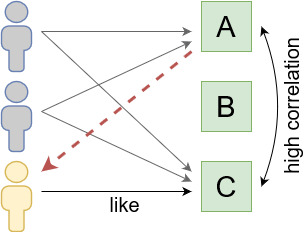
\includegraphics[scale=0.5]{images/IB_CF_ex.PNG}
	\caption{Esempio di applicazione di un sistema di raccomandazione Item-based}
	\label{fig:IB_CF}
\end{figure}

